
% Default to the notebook output style

    


% Inherit from the specified cell style.




    
\documentclass[twocolumn]{article}

    \usepackage{wrapfig}
    \usepackage[font={small}]{caption}
    \usepackage{graphicx} % Used to insert images
    \usepackage{adjustbox} % Used to constrain images to a maximum size 
    \usepackage{color} % Allow colors to be defined
    \usepackage{enumerate} % Needed for markdown enumerations to work
    \usepackage{geometry} % Used to adjust the document margins
    \usepackage{amsmath} % Equations
    \usepackage{amssymb} % Equations
    \usepackage[mathletters]{ucs} % Extended unicode (utf-8) support
    \usepackage[utf8x]{inputenc} % Allow utf-8 characters in the tex document
    \usepackage{fancyvrb} % verbatim replacement that allows latex
    \usepackage{grffile} % extends the file name processing of package graphics 
                         % to support a larger range 
    % The hyperref package gives us a pdf with properly built
    % internal navigation ('pdf bookmarks' for the table of contents,
    % internal cross-reference links, web links for URLs, etc.)
    \usepackage{hyperref}
    \usepackage{longtable} % longtable support required by pandoc >1.10
    \usepackage[russian]{babel}
	\usepackage{dblfloatfix}
	\usepackage{subcaption}
	\usepackage{float}
    \setlength{\parskip}{\baselineskip}%
	\setlength{\parindent}{0pt}%
    
    \definecolor{orange}{cmyk}{0,0.4,0.8,0.2}
    \definecolor{darkorange}{rgb}{.71,0.21,0.01}
    \definecolor{darkgreen}{rgb}{.12,.54,.11}
    \definecolor{myteal}{rgb}{.26, .44, .56}
    \definecolor{gray}{gray}{0.45}
    \definecolor{lightgray}{gray}{.95}
    \definecolor{mediumgray}{gray}{.8}
    \definecolor{inputbackground}{rgb}{.95, .95, .85}
    \definecolor{outputbackground}{rgb}{.95, .95, .95}
    \definecolor{traceback}{rgb}{1, .95, .95}
    % ansi colors
    \definecolor{red}{rgb}{.6,0,0}
    \definecolor{green}{rgb}{0,.65,0}
    \definecolor{brown}{rgb}{0.6,0.6,0}
    \definecolor{blue}{rgb}{0,.145,.698}
    \definecolor{purple}{rgb}{.698,.145,.698}
    \definecolor{cyan}{rgb}{0,.698,.698}
    \definecolor{lightgray}{gray}{0.5}
    
    % bright ansi colors
    \definecolor{darkgray}{gray}{0.25}
    \definecolor{lightred}{rgb}{1.0,0.39,0.28}
    \definecolor{lightgreen}{rgb}{0.48,0.99,0.0}
    \definecolor{lightblue}{rgb}{0.53,0.81,0.92}
    \definecolor{lightpurple}{rgb}{0.87,0.63,0.87}
    \definecolor{lightcyan}{rgb}{0.5,1.0,0.83}
    
    % commands and environments needed by pandoc snippets
    % extracted from the output of `pandoc -s`
    \DefineVerbatimEnvironment{Highlighting}{Verbatim}{commandchars=\\\{\}}
    % Add ',fontsize=\small' for more characters per line
    \newenvironment{Shaded}{}{}
    \newcommand{\KeywordTok}[1]{\textcolor[rgb]{0.00,0.44,0.13}{\textbf{{#1}}}}
    \newcommand{\DataTypeTok}[1]{\textcolor[rgb]{0.56,0.13,0.00}{{#1}}}
    \newcommand{\DecValTok}[1]{\textcolor[rgb]{0.25,0.63,0.44}{{#1}}}
    \newcommand{\BaseNTok}[1]{\textcolor[rgb]{0.25,0.63,0.44}{{#1}}}
    \newcommand{\FloatTok}[1]{\textcolor[rgb]{0.25,0.63,0.44}{{#1}}}
    \newcommand{\CharTok}[1]{\textcolor[rgb]{0.25,0.44,0.63}{{#1}}}
    \newcommand{\StringTok}[1]{\textcolor[rgb]{0.25,0.44,0.63}{{#1}}}
    \newcommand{\CommentTok}[1]{\textcolor[rgb]{0.38,0.63,0.69}{\textit{{#1}}}}
    \newcommand{\OtherTok}[1]{\textcolor[rgb]{0.00,0.44,0.13}{{#1}}}
    \newcommand{\AlertTok}[1]{\textcolor[rgb]{1.00,0.00,0.00}{\textbf{{#1}}}}
    \newcommand{\FunctionTok}[1]{\textcolor[rgb]{0.02,0.16,0.49}{{#1}}}
    \newcommand{\RegionMarkerTok}[1]{{#1}}
    \newcommand{\ErrorTok}[1]{\textcolor[rgb]{1.00,0.00,0.00}{\textbf{{#1}}}}
    \newcommand{\NormalTok}[1]{{#1}}
    
    % Define a nice break command that doesn't care if a line doesn't already
    % exist.
    \def\br{\hspace*{\fill} \\* }
    % Math Jax compatability definitions
    \def\gt{>}
    \def\lt{<}
    % Document parameters
    \title{Исследование неодимового лазера и сопутствующих эффектов}
    \author{Кинзина Э., Федоров Г., Салтыков А., Оразбаев А., Паньков А.}
    
    
    

    % Pygments definitions
    
\makeatletter
\def\PY@reset{\let\PY@it=\relax \let\PY@bf=\relax%
    \let\PY@ul=\relax \let\PY@tc=\relax%
    \let\PY@bc=\relax \let\PY@ff=\relax}
\def\PY@tok#1{\csname PY@tok@#1\endcsname}
\def\PY@toks#1+{\ifx\relax#1\empty\else%
    \PY@tok{#1}\expandafter\PY@toks\fi}
\def\PY@do#1{\PY@bc{\PY@tc{\PY@ul{%
    \PY@it{\PY@bf{\PY@ff{#1}}}}}}}
\def\PY#1#2{\PY@reset\PY@toks#1+\relax+\PY@do{#2}}

\expandafter\def\csname PY@tok@nl\endcsname{\def\PY@tc##1{\textcolor[rgb]{0.63,0.63,0.00}{##1}}}
\expandafter\def\csname PY@tok@nn\endcsname{\let\PY@bf=\textbf\def\PY@tc##1{\textcolor[rgb]{0.00,0.00,1.00}{##1}}}
\expandafter\def\csname PY@tok@sx\endcsname{\def\PY@tc##1{\textcolor[rgb]{0.00,0.50,0.00}{##1}}}
\expandafter\def\csname PY@tok@ni\endcsname{\let\PY@bf=\textbf\def\PY@tc##1{\textcolor[rgb]{0.60,0.60,0.60}{##1}}}
\expandafter\def\csname PY@tok@ss\endcsname{\def\PY@tc##1{\textcolor[rgb]{0.10,0.09,0.49}{##1}}}
\expandafter\def\csname PY@tok@ne\endcsname{\let\PY@bf=\textbf\def\PY@tc##1{\textcolor[rgb]{0.82,0.25,0.23}{##1}}}
\expandafter\def\csname PY@tok@nf\endcsname{\def\PY@tc##1{\textcolor[rgb]{0.00,0.00,1.00}{##1}}}
\expandafter\def\csname PY@tok@kd\endcsname{\let\PY@bf=\textbf\def\PY@tc##1{\textcolor[rgb]{0.00,0.50,0.00}{##1}}}
\expandafter\def\csname PY@tok@na\endcsname{\def\PY@tc##1{\textcolor[rgb]{0.49,0.56,0.16}{##1}}}
\expandafter\def\csname PY@tok@nb\endcsname{\def\PY@tc##1{\textcolor[rgb]{0.00,0.50,0.00}{##1}}}
\expandafter\def\csname PY@tok@nc\endcsname{\let\PY@bf=\textbf\def\PY@tc##1{\textcolor[rgb]{0.00,0.00,1.00}{##1}}}
\expandafter\def\csname PY@tok@k\endcsname{\let\PY@bf=\textbf\def\PY@tc##1{\textcolor[rgb]{0.00,0.50,0.00}{##1}}}
\expandafter\def\csname PY@tok@nt\endcsname{\let\PY@bf=\textbf\def\PY@tc##1{\textcolor[rgb]{0.00,0.50,0.00}{##1}}}
\expandafter\def\csname PY@tok@si\endcsname{\let\PY@bf=\textbf\def\PY@tc##1{\textcolor[rgb]{0.73,0.40,0.53}{##1}}}
\expandafter\def\csname PY@tok@no\endcsname{\def\PY@tc##1{\textcolor[rgb]{0.53,0.00,0.00}{##1}}}
\expandafter\def\csname PY@tok@gi\endcsname{\def\PY@tc##1{\textcolor[rgb]{0.00,0.63,0.00}{##1}}}
\expandafter\def\csname PY@tok@sc\endcsname{\def\PY@tc##1{\textcolor[rgb]{0.73,0.13,0.13}{##1}}}
\expandafter\def\csname PY@tok@sb\endcsname{\def\PY@tc##1{\textcolor[rgb]{0.73,0.13,0.13}{##1}}}
\expandafter\def\csname PY@tok@nv\endcsname{\def\PY@tc##1{\textcolor[rgb]{0.10,0.09,0.49}{##1}}}
\expandafter\def\csname PY@tok@se\endcsname{\let\PY@bf=\textbf\def\PY@tc##1{\textcolor[rgb]{0.73,0.40,0.13}{##1}}}
\expandafter\def\csname PY@tok@sd\endcsname{\let\PY@it=\textit\def\PY@tc##1{\textcolor[rgb]{0.73,0.13,0.13}{##1}}}
\expandafter\def\csname PY@tok@err\endcsname{\def\PY@bc##1{\setlength{\fboxsep}{0pt}\fcolorbox[rgb]{1.00,0.00,0.00}{1,1,1}{\strut ##1}}}
\expandafter\def\csname PY@tok@vi\endcsname{\def\PY@tc##1{\textcolor[rgb]{0.10,0.09,0.49}{##1}}}
\expandafter\def\csname PY@tok@nd\endcsname{\def\PY@tc##1{\textcolor[rgb]{0.67,0.13,1.00}{##1}}}
\expandafter\def\csname PY@tok@gt\endcsname{\def\PY@tc##1{\textcolor[rgb]{0.00,0.27,0.87}{##1}}}
\expandafter\def\csname PY@tok@sr\endcsname{\def\PY@tc##1{\textcolor[rgb]{0.73,0.40,0.53}{##1}}}
\expandafter\def\csname PY@tok@bp\endcsname{\def\PY@tc##1{\textcolor[rgb]{0.00,0.50,0.00}{##1}}}
\expandafter\def\csname PY@tok@c1\endcsname{\let\PY@it=\textit\def\PY@tc##1{\textcolor[rgb]{0.25,0.50,0.50}{##1}}}
\expandafter\def\csname PY@tok@s1\endcsname{\def\PY@tc##1{\textcolor[rgb]{0.73,0.13,0.13}{##1}}}
\expandafter\def\csname PY@tok@kr\endcsname{\let\PY@bf=\textbf\def\PY@tc##1{\textcolor[rgb]{0.00,0.50,0.00}{##1}}}
\expandafter\def\csname PY@tok@mf\endcsname{\def\PY@tc##1{\textcolor[rgb]{0.40,0.40,0.40}{##1}}}
\expandafter\def\csname PY@tok@il\endcsname{\def\PY@tc##1{\textcolor[rgb]{0.40,0.40,0.40}{##1}}}
\expandafter\def\csname PY@tok@kt\endcsname{\def\PY@tc##1{\textcolor[rgb]{0.69,0.00,0.25}{##1}}}
\expandafter\def\csname PY@tok@s2\endcsname{\def\PY@tc##1{\textcolor[rgb]{0.73,0.13,0.13}{##1}}}
\expandafter\def\csname PY@tok@mo\endcsname{\def\PY@tc##1{\textcolor[rgb]{0.40,0.40,0.40}{##1}}}
\expandafter\def\csname PY@tok@mi\endcsname{\def\PY@tc##1{\textcolor[rgb]{0.40,0.40,0.40}{##1}}}
\expandafter\def\csname PY@tok@mh\endcsname{\def\PY@tc##1{\textcolor[rgb]{0.40,0.40,0.40}{##1}}}
\expandafter\def\csname PY@tok@kc\endcsname{\let\PY@bf=\textbf\def\PY@tc##1{\textcolor[rgb]{0.00,0.50,0.00}{##1}}}
\expandafter\def\csname PY@tok@vg\endcsname{\def\PY@tc##1{\textcolor[rgb]{0.10,0.09,0.49}{##1}}}
\expandafter\def\csname PY@tok@vc\endcsname{\def\PY@tc##1{\textcolor[rgb]{0.10,0.09,0.49}{##1}}}
\expandafter\def\csname PY@tok@ow\endcsname{\let\PY@bf=\textbf\def\PY@tc##1{\textcolor[rgb]{0.67,0.13,1.00}{##1}}}
\expandafter\def\csname PY@tok@kn\endcsname{\let\PY@bf=\textbf\def\PY@tc##1{\textcolor[rgb]{0.00,0.50,0.00}{##1}}}
\expandafter\def\csname PY@tok@ge\endcsname{\let\PY@it=\textit}
\expandafter\def\csname PY@tok@gd\endcsname{\def\PY@tc##1{\textcolor[rgb]{0.63,0.00,0.00}{##1}}}
\expandafter\def\csname PY@tok@m\endcsname{\def\PY@tc##1{\textcolor[rgb]{0.40,0.40,0.40}{##1}}}
\expandafter\def\csname PY@tok@o\endcsname{\def\PY@tc##1{\textcolor[rgb]{0.40,0.40,0.40}{##1}}}
\expandafter\def\csname PY@tok@cm\endcsname{\let\PY@it=\textit\def\PY@tc##1{\textcolor[rgb]{0.25,0.50,0.50}{##1}}}
\expandafter\def\csname PY@tok@go\endcsname{\def\PY@tc##1{\textcolor[rgb]{0.53,0.53,0.53}{##1}}}
\expandafter\def\csname PY@tok@c\endcsname{\let\PY@it=\textit\def\PY@tc##1{\textcolor[rgb]{0.25,0.50,0.50}{##1}}}
\expandafter\def\csname PY@tok@kp\endcsname{\def\PY@tc##1{\textcolor[rgb]{0.00,0.50,0.00}{##1}}}
\expandafter\def\csname PY@tok@gh\endcsname{\let\PY@bf=\textbf\def\PY@tc##1{\textcolor[rgb]{0.00,0.00,0.50}{##1}}}
\expandafter\def\csname PY@tok@gu\endcsname{\let\PY@bf=\textbf\def\PY@tc##1{\textcolor[rgb]{0.50,0.00,0.50}{##1}}}
\expandafter\def\csname PY@tok@sh\endcsname{\def\PY@tc##1{\textcolor[rgb]{0.73,0.13,0.13}{##1}}}
\expandafter\def\csname PY@tok@gs\endcsname{\let\PY@bf=\textbf}
\expandafter\def\csname PY@tok@gr\endcsname{\def\PY@tc##1{\textcolor[rgb]{1.00,0.00,0.00}{##1}}}
\expandafter\def\csname PY@tok@gp\endcsname{\let\PY@bf=\textbf\def\PY@tc##1{\textcolor[rgb]{0.00,0.00,0.50}{##1}}}
\expandafter\def\csname PY@tok@cs\endcsname{\let\PY@it=\textit\def\PY@tc##1{\textcolor[rgb]{0.25,0.50,0.50}{##1}}}
\expandafter\def\csname PY@tok@s\endcsname{\def\PY@tc##1{\textcolor[rgb]{0.73,0.13,0.13}{##1}}}
\expandafter\def\csname PY@tok@cp\endcsname{\def\PY@tc##1{\textcolor[rgb]{0.74,0.48,0.00}{##1}}}
\expandafter\def\csname PY@tok@w\endcsname{\def\PY@tc##1{\textcolor[rgb]{0.73,0.73,0.73}{##1}}}

\def\PYZbs{\char`\\}
\def\PYZus{\char`\_}
\def\PYZob{\char`\{}
\def\PYZcb{\char`\}}
\def\PYZca{\char`\^}
\def\PYZam{\char`\&}
\def\PYZlt{\char`\<}
\def\PYZgt{\char`\>}
\def\PYZsh{\char`\#}
\def\PYZpc{\char`\%}
\def\PYZdl{\char`\$}
\def\PYZhy{\char`\-}
\def\PYZsq{\char`\'}
\def\PYZdq{\char`\"}
\def\PYZti{\char`\~}
% for compatibility with earlier versions
\def\PYZat{@}
\def\PYZlb{[}
\def\PYZrb{]}
\makeatother


    % Exact colors from NB
    \definecolor{incolor}{rgb}{0.0, 0.0, 0.5}
    \definecolor{outcolor}{rgb}{0.545, 0.0, 0.0}



    
    % Prevent overflowing lines due to hard-to-break entities
    \sloppy 
    % Setup hyperref package
    \hypersetup{
      breaklinks=true,  % so long urls are correctly broken across lines
      colorlinks=true,
      urlcolor=blue,
      linkcolor=darkorange,
      citecolor=darkgreen,
      }
    % Slightly bigger margins than the latex defaults
    
    \geometry{verbose,tmargin=1in,bmargin=1in,lmargin=1in,rmargin=1in}
    
    \raggedbottom

    \begin{document}

        
            \maketitle
       

    
\section*{Содержание}
\begin{enumerate}
\def\labelenumi{\arabic{enumi}.}
\item
  Принципы работы квантового генератора
\item
  Неодимовый лазер
    \begin{enumerate}[{2.}1]
    
	\item
  Общая схема установки
  \item
  Подготовка к работе
	\item
  Люминисценция кристалла
	\item
  Лазерная генерация
	\item
  Энергия и форма импульса лазерной генерации
  \end{enumerate}
\item
  Неодимовый лазер с модулированной добротностью
    \begin{enumerate}[{3.}1]

	\item
  Нелинейные поглотители
	\item
  Энергия импульса
	\item
  Форма импульсов
	\item
  Пробой воздуха
  \end{enumerate}
\item
  Вторая гармоника
    \begin{enumerate}[{4.}1]

	\item
  Теоретическое введение
	\item
  Результаты
  \end{enumerate}
\item
  Приложения
    \begin{enumerate}[{5.}1]

	\item
  Осциллограммы, не вошедшие в основной отчет
  
	\item
  Спектры, не вошедшие в основной отчет
  \end{enumerate}
\end{enumerate}
\section{Принципы работы квантового генератора}Лазерный излучатель, служащий для генерации электромагнитного излучения
оптического диапазона с уникальными свойствами, структурно состоит из
следующих основных элементов: активной среды, источника накачки и
резонатора.$\newline$ Активная среда − это вещество, в котором может
быть создана инверсная населённость энергетических уровней, т.е.
достигнуто такое состояние, когда число атомов, находящихся на верхнем
``рабочем'' энергетическом уровне, превышает число атомов, находящихся
на нижнем ``рабочем'' энергетическом уровне. По типу активной среды
лазеры подразделяются на твердотельные, газовые, полупроводниковые,
жидкостные и др. На практике активную среду твердотельных лазеров часто
также называют активным элементом.$\newline$ Поставщиком энергии для
достижения состояния инверсной населённости служит источник накачки, в
качестве которого может выступать, например: лампа−вспышка, газовый
разряд, инжекция носителей тока в полупроводниковых p−n переходах,
тепловой способ, химическая реакция и др.$\newline$ Важнейшей и
неотъемлемой частью любого лазера является резонатор − система,
состоящая, как правило, из двух отражающих поверхностей, между которыми
располагается активная среда.$\newline$ Отражающие поверхности могут
представлять собой зеркала различной формы (плоские, сферические,
параболические и др.), грани призм полного внутреннего отражения или
границы раздела сред с различными показателями преломления.$\newline$
Зеркала лазера чаще всего формируются путём нанесения многослойных
отражающих диэлектрических покрытий на одну из отполированных по
специальной технологии поверхностей основы зеркала − на так называемую
подложку. На другую поверхность подложки зеркала либо наносят
просветляющее покрытие, либо её оставляют без покрытия. Поверхность
зеркала с отражающим покрытием называется ``рабочей'', одно из зеркал
резонатора, полностью отражающее свет, − ``глухим'', а зеркало, частично
пропускающее излучение, − выходным. Основным назначением оптического
резонатора является создание условий, при которых возникающее в активной
среде излучение, многократно проходя через её структуру, усиливается до
уровня превышения имеющихся потерь. Следовательно, резонатор
осуществляет положительную обратную связь. Другим его немаловажным

Самым простым и наиболее распространённым видом резонатора является система из
двух плоских зеркал, обращённых друг к другу отражающими поверхностями,
называемая эталоном Фабри−Перо. 

Под юстировкой системы в общем случае
понимают совокупность операций по приведению её элементов в состояние,
обеспечивающее правильное функционирование системы.

Под режимом свободной генерации лазера понимают такой режим, при котором
отсутствует какое−либо целенаправленное управление параметрами или
элементами лазерного излучателя в процессе генерации. Так как в режиме
свободной генерации отсутствуют дополнительные потери излучения в
резонаторе на элементах управления, то лазеры имеют здесь наибольшую
энергию импульса генерации. Соответственно, в этом режиме лазер обладает
и наибольшим коэффициентом полезного действия − КПД. 
\section{Неодимовый лазер}
\subsection{Общая схема установки}

Неодимовый лазер - частный случай твердотельного лазера, в качестве активной среды которого используется  алюмо-иттриевый гранат («YAG», $Y_3Al_5O_{12}$) легированный ионами неодима (Nd).

Генерация происходит на длине волны 1064 нм. Такие лазеры могут работать как в непрерывном, так и в импульсном режиме. Импульсные режимы отличаются характером генерации лазерного излучения. В свободной генерации длительность импульса обычно равна времени жизни верхнего лазерного уровня (около 250 мкс, зависит от концентрации неодима), импульс представляет собой набор пичков с длительностью до сотен наносекунд. В режиме модулированной добротности длительность может варьироваться от единиц наносекунд до микросекунд. Наибольшую импульсную мощность можно получить при работе в режиме модуляции добротности. Благодаря большой мощности, из импульса с длиной волны 1064 нм на нелинейном кристалле можно получить импульс с длиной волны вдвое, втрое, вчетверо (и т. д.) короче, например: 532 нм, 355 нм, 266 нм, 213 нм. В лазере используется четырехуровневая накачка (Рис. \ref{fig:levels}), рабочий переход - с терма $^4F_{3/2}$ на терм $^4I_{11/2}$.

\begin{figure}
\centering
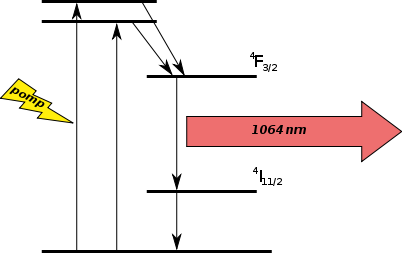
\includegraphics[width=0.4\textwidth]{LEMPH Report_files/levels.png}
\caption{Четырехуровневая накачка (верхний уровень расщеплен) \label{fig:levels}}

\end{figure}

\begin{figure}
\centering
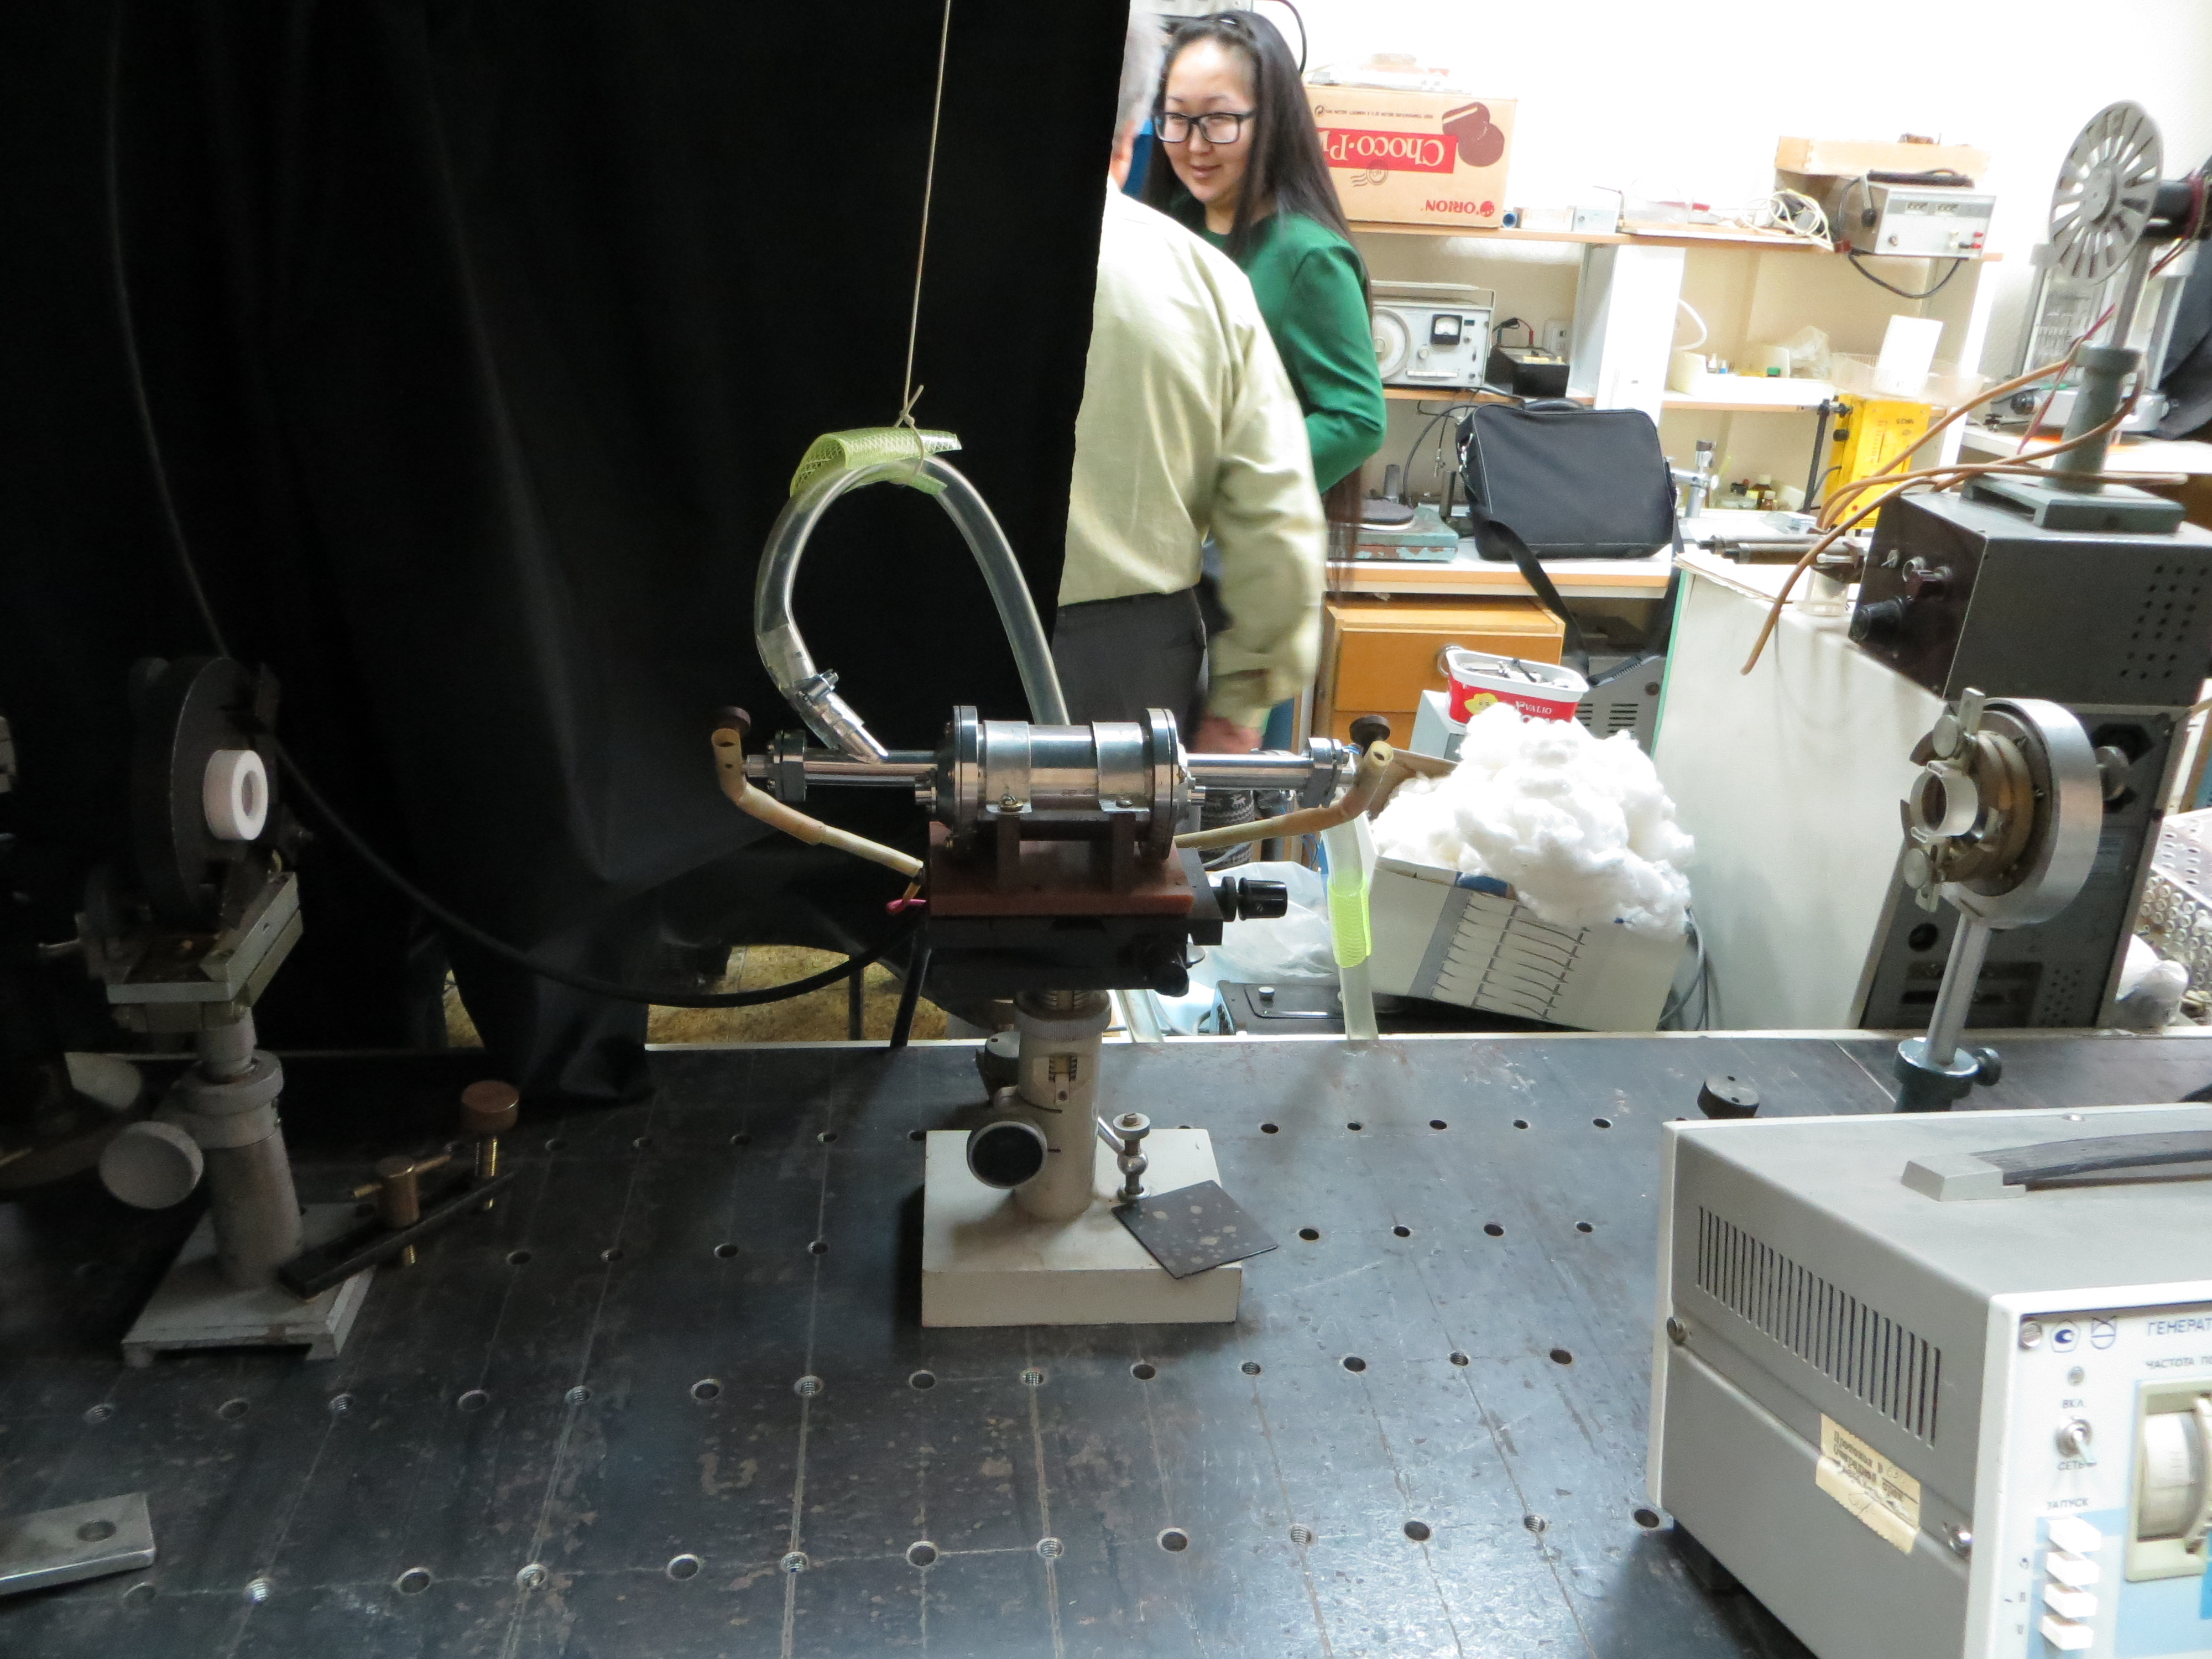
\includegraphics[width=0.4\textwidth]{LEMPH Report_files/apparatus.JPG}
\caption{По центру - упакованные в металлический кожух кристалл и лампа-вспышка, слева и справа - зеркала резонатора \label{fig:apparatus}}
\end{figure}

Схема установки в экспериментах являлась классической, на основе интерферометра Фабри-Перо. Фото лабораторной установки приведено на Рис. \ref{fig:apparatus}. В качестве резонатора использовались зеркала со следующими коэффициентами отражения: левое (глухое) - 98\%, правое (выходное) - 90\%. Для охлаждения рабочего тела применялась и применяется жидкостная схема, которая, к сожалению, является на данный момент очень ненадежной. Накачка лазера осуществлялась лампой-вспышкой, подключенной к источнику высокого напряжения, затравочный разряд для ее запуска производился генератором импульсов.

Целью работы на данном этапе было получение генерации и измерение различных параметров, таких как длина волны излучения лазера, спектры излучения и люминисцентного свечения кристалла (до-генерационный режим), а также временные диаграммы интенсивности излучения.

\subsection{Подготовка к работе}
Прежде всего было необходимо провести юстировку лазера. Под юстировкой системы в общем случае
понимают совокупность операций по приведению её элементов в состояние,
обеспечивающее правильное функционирование системы. Юстировка
оптических систем заключается в регулировании взаимного расположения
оптических деталей (линз, призм, зеркал и т.п.) с целью их центрирования
и обеспечения наилучшего качества изображения. В съюстированном
положении оптические детали закрепляются винтами, штифтами либо
склеиваются.Физический смысл процесса юстировки лазера
состоит в нахождении такого расположения его оптических элементов
(активной среды, зеркал резонатора и т.п.) друг относительно друга, при
котором потери излучения минимальны.

На практике юстировку разделяют на ``холодную'' (или грубую) и ``горячую'' (или
тонкую). В первом случае широкое практическое применение
получил метод так называемого оптического рычага, для реализации
которого необходим вспомогательный юстировочный лазер − низкоинтенсивный
лазер, генерирующий излучение в видимом диапазоне. Источник же накачки
юстируемого лазера в этом случае не включается.``Горячая''
юстировка осуществляется уже при непосредственном включении источника
накачки юстируемого лазера, что позволяет учесть термооптические
особенности настраиваемой системы. Данный вид юстировки производится с
использованием специальных средств, в качестве которых обычно выступают:
визуализаторы и регистраторы излучения (например, копировальная бумага,
фотобумага и др.), фотоприёмник, измеритель энергии/мощности лазерного
излучения и др. Для оценки степени чувствительности лазерного
резонатора к разъюстировке служит разъюстировочная характеристика,
представляющая собой зависимость параметров лазерной генерации от угла
отклонения одного из зеркал резонатора относительно съюстированного
положения.

Для получения максимальной мощности пучка при минимальной расходимости
были использован следующий порядок действий (все цифровые обозначения отвечают Рис. \ref{fig:justify}):
\subsubsection{\emph{Холодная юстировка}}
\begin{enumerate}
\def\labelenumi{\arabic{enumi}.}
\item
  Включить вспомогательный юстировочный лазер \textbf{1}. Его луч должен
  пройти через отверстие в юстировочной диафрагме \textbf{2}.
\item
  Установить на пути следования луча от вспомогательного юстировочного
  лазера \textbf{1} активный элемент \textbf{6} юстируемого лазера таким
  образом, чтобы луч от вспомогательного лазера \textbf{1} проходил
  вдоль его оси через центр. Позиционирование проводить с помощью
  юстировочных винтов оптической подвижки, в которой закреплён
  юстируемый активный элемент \textbf{6}. Контроль за прохождением луча
  от вспомогательного юстировочного лазера \textbf{1} осуществлять
  визуально.
\item
  Посредством юстировочных винтов подвижки активного элемента
  \textbf{6}, ответственных за угловые перемещения объекта, добиться
  наиболее точного совпадения блика (светового отражения) от входного
  торца активного элемента \textbf{6} с отверстием диафрагмы \textbf{2}.
\item
  На выходе из активного элемента \textbf{6} проверить ещё раз качество
  излучения от вспомогательного юстировочного лазера \textbf{1}.
\item
  Найти на экране \textbf{8} блик от входного торца активного элемента
  \textbf{6}.
\item
  Зафиксировать на экране \textbf{8} местоположение блика от входного
  торца активного элемента \textbf{6} (см. рис. 1.1).
\item
  Не сбивая юстировки активного элемента \textbf{6}, установить на пути
  следования луча от вспомогательного юстировочного лазера \textbf{1}
  выходное зеркало \textbf{7} резонатора таким образом, чтобы данный луч
  проходил примерно через его центр. Подобная установка осуществляется с
  помощью юстировочных винтов оптической подвижки, ответственных за
  линейные перемещения объекта.
\item
  Наблюдая за экраном \textbf{8}, посредством юстировочных винтов
  подвижки выходного зеркала \textbf{7}, ответственных за угловые
  перемещения объекта, совместить блик от его поверхности с
  местоположением блика от входного торца активного элемента \textbf{6}
  (см. рис. 1.1).
\item
  Повторить все действия из п. 8 и п. 9 для ``глухого'' зеркала
  \textbf{5} резонатора.
\end{enumerate}
\subsubsection{\emph{Горячая юстировка}}
\begin{enumerate}
\def\labelenumi{\arabic{enumi}.}
\itemsep1pt\parskip0pt\parsep0pt
\item
  Установить на выходе из съюстированного в результате выполнения
  предыдущего задания лазерного излучателя фрагмент фотобумаги −
  объект−мишень \textbf{9}.
\item
  По виду ожога, полученного на фотобумаге, оценить качество выполненной
  ранее ``холодной'' юстировки.
\item
  Продолжая использовать фотобумагу, путём незначительного вращения
  юстировочных винтов подвижки активного элемента \textbf{6}, отвечающих
  за угловые перемещения объекта, провести его доюстировку.
\item
  По аналогии с предыдущим пунктом провести доюстировку выходного
  \textbf{7} и ``глухого'' \textbf{5} зеркал резонатора.
\end{enumerate}

 
         
    \begin{figure}
    \centering
    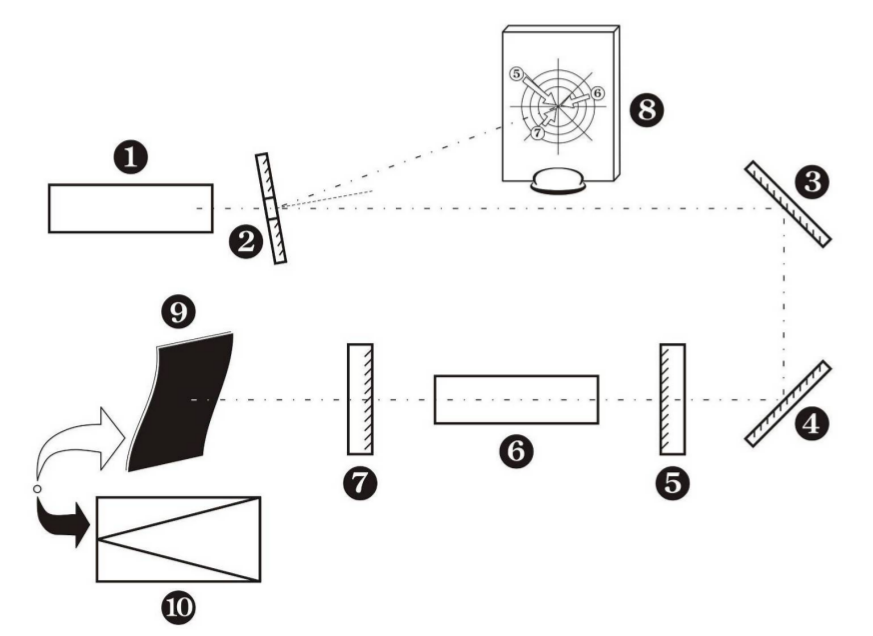
\includegraphics[width=0.4\textwidth]{LEMPH Report_files/LEMPH Report_14_0.png}
    \caption{К действиям при юстировке \label{fig:justify}}
    \end{figure}
               
        

    
\subsection{Люминесценция кристалла}

Для измерения спектров в работе применялся работающий на основе ПЗС-матрицы мини-спектрометр FSD-9. На примере излучения красного гелий-неонового лазера можно оценить его разрешающую способность (Рис. \ref{fig:red_lasar}). Действительно, для гелий-неоновых лазеров типичная спектральная ширина линии составляет порядка 1 ГГц, по формуле $|\Delta \lambda| = |\Delta \nu \frac{\lambda^2}{c}|$ получаем для $\lambda$=630 нм ширину $\sim$ 0.003 нм, что гораздо меньше величины, определяемой спектрометром.
Спектр люминисценции имеет вид, представленный на Рис. \ref{fig:lumina_spectrum}, при напряжении на питающем конденсаторе в 1.5 кВ

\begin{figure}[h!]
	\centering
	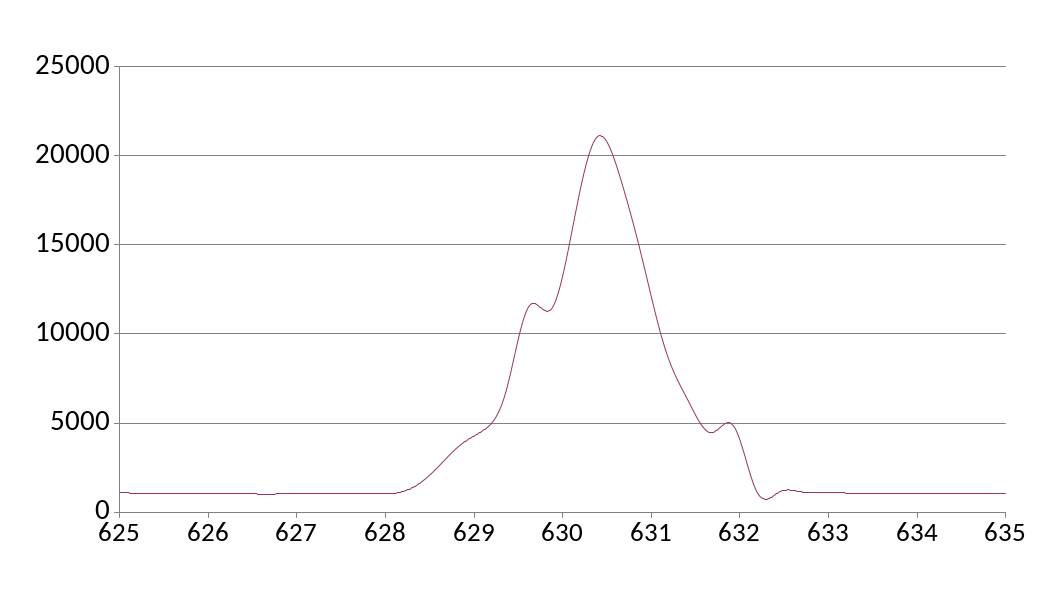
\includegraphics[width=0.5\textwidth]{LEMPH Report_files/red_lasar.png}
	\caption{Измеренный спектр гелий-неонового лазера. На самом деле ширина линии составляет несколько 				тысячных нанометра \label{fig:red_lasar}}
\end{figure}
    
        
\begin{figure}
	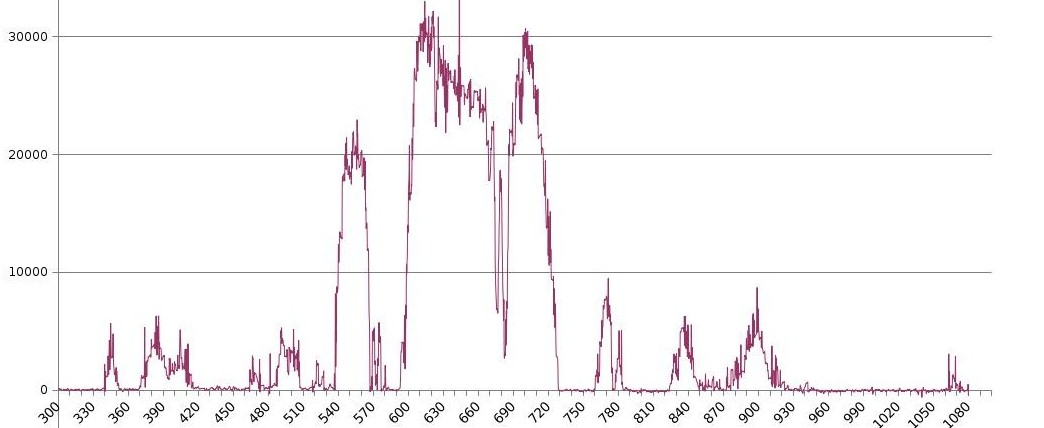
\includegraphics[width=0.5\textwidth]{LEMPH Report_files/LEMPH Report_17_0.jpeg}
	\caption{Спектр люминисценции кристалла при напряжении 1.5 кВ. Из-за несовершенства спектрометра не 			видно, что максимальная интенсивность приходится на 1064 нм, но так и есть \label{fig:lumina_spectrum}}
\end{figure}
           
Для снятия временных диаграмм использовался фотодиод, самодельный. \emph{Его} разрешающая способность(по времени) будет продемонстрирована ниже при рассмотрении режима с модцлированной добротностью.
Подавая сигнал с фотодиода (при попадании на него света люминисценции) на вход цифрового осциллографа, получили следующую осциллограмму, форму импульса во времени, опять же для 1.5 кВ (Рис. \ref{fig:lumina_pulse})

   
    \begin{figure}[h!]
    \centering
    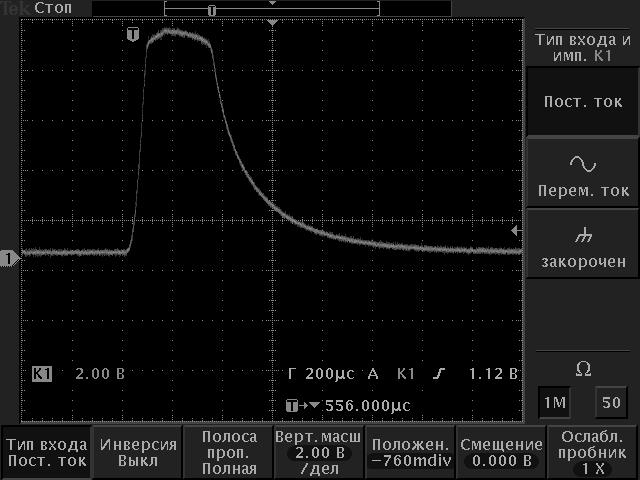
\includegraphics[width=0.4\textwidth]{LEMPH Report_files/LEMPH Report_19_0.jpeg}
    \caption{Форма импульса люминисценции в времени, 1.5 кВ \label{fig:lumina_pulse}}
    \end{figure}
    
          
        
    
\subsection{Генерация}
В результате проведенной подготовки (в основном благодаря "холодной" юстировке) была получена генерация в свободном режиме. 

\subsubsection{Пороговая энергия}
Генерация в лазере может наблюдаться не всегда. Требуется выполнение условия преобладания закачиваемой энергии над потерями в процессе усиления. Математически можно это записать следующим образом: усиление при прохождении через активную среду должно быть больше в первом приближении чем потери при отражении от зеркал:
\begin{align*}
J_0\ (e^{\alpha(\omega_0)\ x}-1) \geq J_0\ (0.02+0.1)
\end{align*}
Было проведено исследование работы лазера при различных энергиях
накачки. Для этого использовался измеритель средней мощности и энергии лазерного излучения ИМО-2Н. В результате был получен следующий график зависимости интегральной
энергии импульса от энергии накачки (Рис. \ref{fig:pulse_over_pomp_energy}). 
Экстраполируя полученные точки можно получить значение пороговой энергии накачки - она составляет примерно 14.9 Дж. 
        
    \begin{figure}
    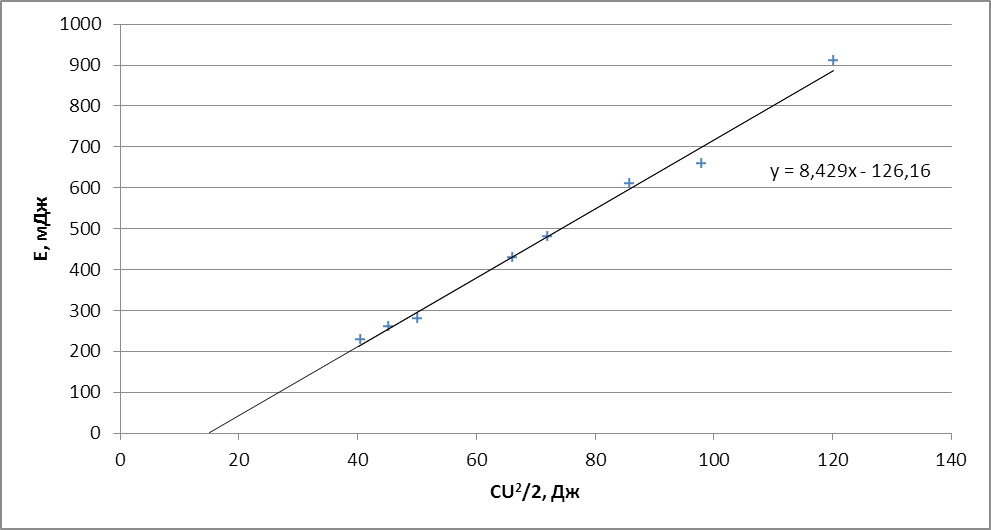
\includegraphics[width=0.5\textwidth]{LEMPH Report_files/LEMPH Report_22_0.png}
    \caption{Зависимость энергии излучения от энергии накачки \label{fig:pulse_over_pomp_energy}}
    \end{figure}
    
            
        
    

\subsubsection{Спектр}
Спектр рассеянного излучения лазера на неодиме. Отчетливо видна длина
волны, на которой происходит генерация - 1064 нм (Рис. \ref{fig:generation_spectrum})

  
    
     
    \begin{figure}
	\centering
    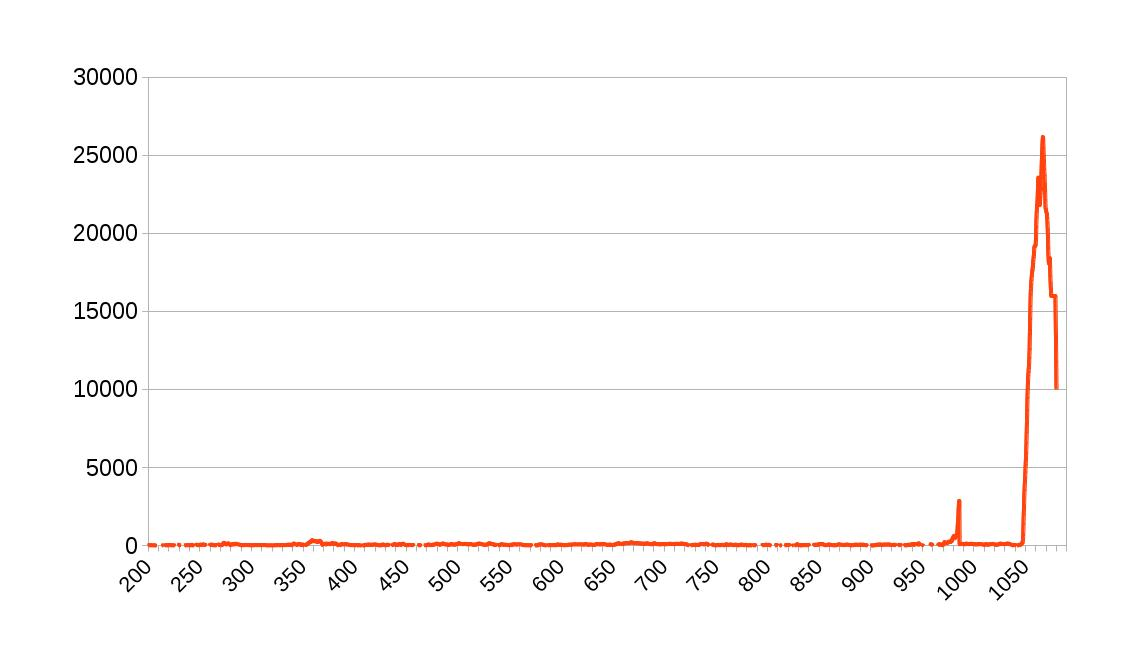
\includegraphics[width=0.5\textwidth]{LEMPH Report_files/LEMPH Report_26_0.jpeg}
    \caption{Спектр генерации \label{fig:generation_spectrum}}
    \end{figure}
    
            
        
    
\subsubsection{Форма импульса}
Подавая сигнал с фотодиода (при освещении его рассеянным светом от
лазерного луча) на вход цифрового осциллографа, получили следующую
осциллограмму (Рис. \ref{fig:laser_pulse})

    
      
    \begin{figure}
    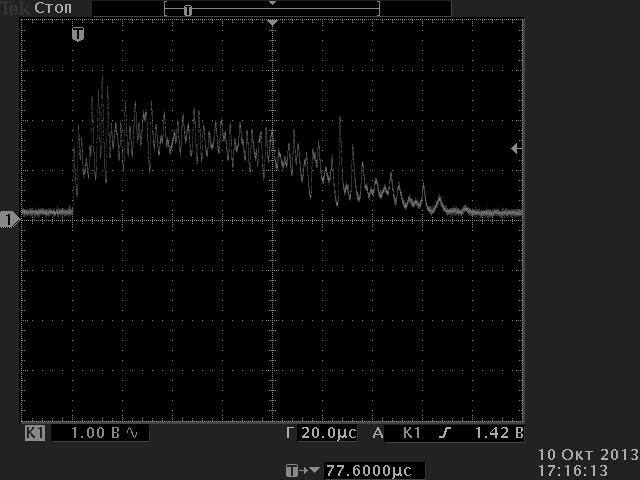
\includegraphics[width=0.5\textwidth]{LEMPH Report_files/LEMPH Report_29_0.jpeg}
    \caption{Форма испульса для генерации \label{fig:laser_pulse}}
    \end{figure}
    
         
            
        
    
\section{Неодимовый лазер с модулированной добротностью}
\subsection{Нелинейные поглотители}
Режим модуляции добротности твердотельного лазера служит для получения
мощного импульса малой длительности (1÷100 нс) или последовательности
таких импульсов. От режима свободной генерации он отличается тем, что
при нём первоначально с помощью внутрирезонаторного затвора
устанавливается малая добротность резонатора (большой уровень потерь).
Поскольку условия для возникновения генерации в лазере в этом случае не
выполняются, то под действием источника накачки в активном элементе
происходит значительное увеличение количества атомов на верхнем
``рабочем'' уровне. Если же теперь в некоторый момент времени быстро
переключить внутрирезонаторный затвор (т.е. увеличить добротность
резонатора), то коэффициент усиления излучения в резонаторе будет
значительно превышать остаточный уровень потерь. Именно это условие и
отличает работу лазера в режиме модулированной добротности от лазера,
работающего в режиме свободной генерации. Большое начальное значение
коэффициента усиления в режиме модулированной добротности по сравнению с
режимом свободной генерации приводит к уменьшению времени развития
импульса излучения, сокращению его длительности и увеличению мощности.
Энергия же одиночного импульса в режиме модулированной добротности из−за
присутствия в резонаторе источника дополнительных потерь
(внутрирезонаторного затвора), как правило, меньше, чем в режиме
свободной генерации.

\subsection{Энергия импульса}

Для получения короткого мощного импульса использовались нелинейные
поглотители. Нелинейный поглотитель имеет низкий коэффициент пропускания при малых интенсивностях падающего излучения, но при их увеличении ситуация меняется, и поглотитель переходит в пропускающий режим. Это утверждение было проверено на практике, и получен соответствующий график коэффициента пропускания в зависимости от падающей энергии (Рис. \ref{fig:nrj_pogl}). Как видно, поглотитель действительно нелинейный, но до мощностей, в которых он практически не пропускает мы не дошли. Впрочем, это и понятно, так как при зарождении генерации энергия падающего на поглотитель излучения, конечно, меньше, чем у использованных нами в эксперименте импульсов, а это именна та область, где должен находиться его порог.

 
    \begin{figure}
    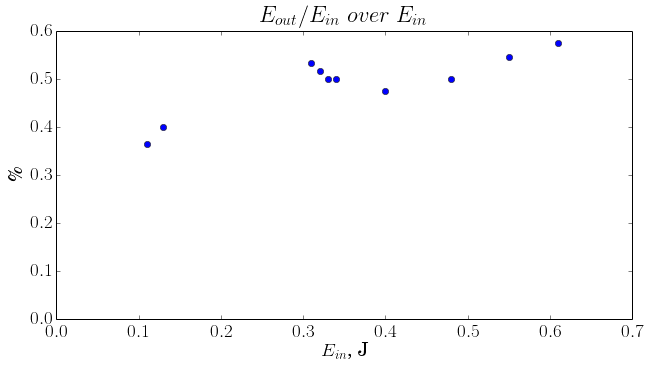
\includegraphics[width=0.5\textwidth]{LEMPH Report_files/nrj_graph.png}
    \caption{Коэффициент пропускания в зависимости от энергии падающего пучка \label{fig:nrj_pogl}}
    \end{figure}
    

    
\subsection{Форма импульсов}

    
 Была получена также и осциллограмма импульсов. На Рис. \ref{fig:mq_osc} видно, что измеренная длительность импульсов составляет порядка 5 мкс. На самом деле длительность сильно завышена измерительным прибором. Это было доказано с использованием лазера, испускающего импульсы достоверно известной наносекундной длительности.
 \begin{figure}
    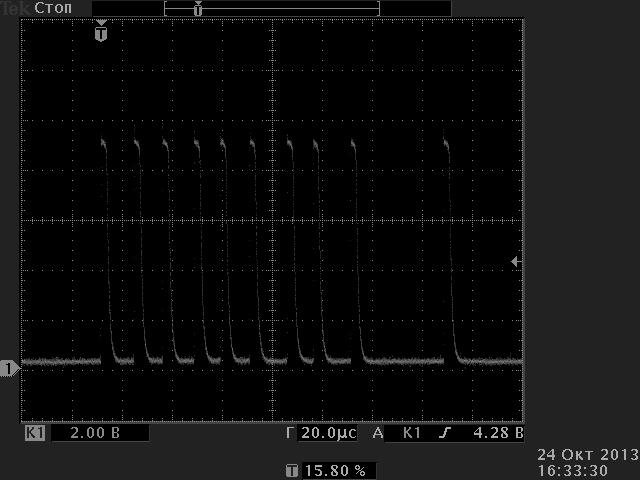
\includegraphics[width=0.5\textwidth]{LEMPH Report_files/LEMPH Report_37_0.jpeg}
    \caption{Форма импульсов наносекундной длительности (на осциллограмме длительность сильно завышена в силу небольшой разрешающей способности детектора) \label{fig:mq_osc}}
    \end{figure}
    
          \newpage  
        
    
\subsection{Пробой воздуха}Полученной мощности хватило для лазерного пробоя воздуха (Рис. \ref{fig:strike})

    % Make sure that atleast 4 lines are below the HR

    
       
    \begin{figure}
    \centering
    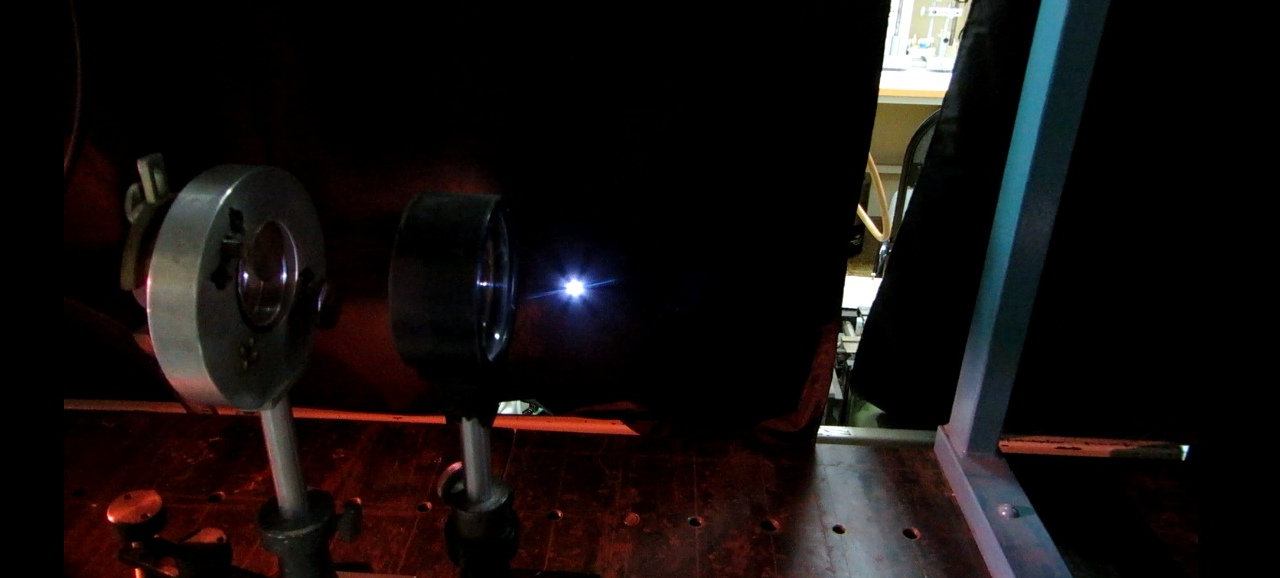
\includegraphics[width=0.4\textwidth]{LEMPH Report_files/LEMPH Report_40_0.jpeg}
    \caption{Пробой воздуха невооруженным глазом \label{fig:strike}}
    \end{figure}
    
        
        
    
Удалось так же снять спектр вспышки, которая видна на рисунке. Он имеет
следующий вид (Рис. \ref{fig:boom_spectrum})

    % Make sure that atleast 4 lines are below the HR

    
      
    \begin{figure}
    \centering
    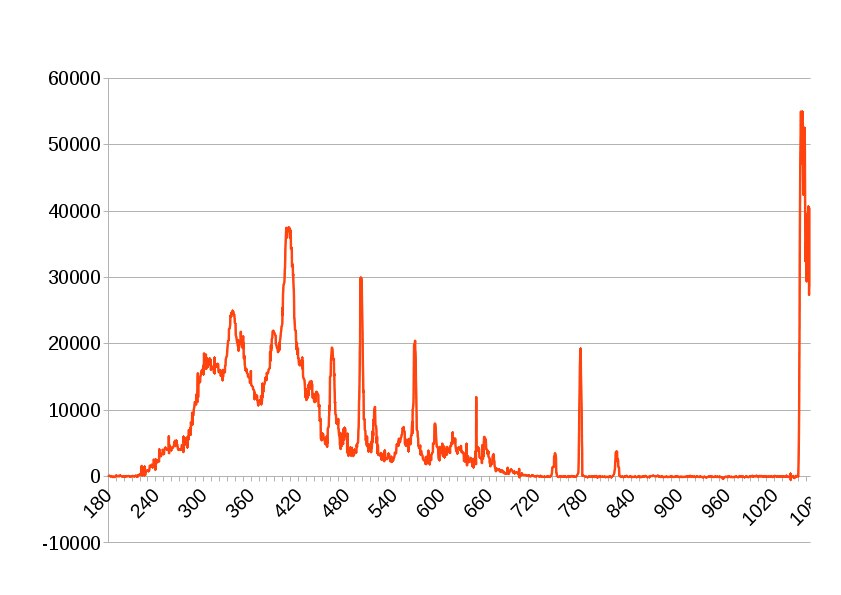
\includegraphics[width=0.4\textwidth]{LEMPH Report_files/LEMPH Report_42_0.jpeg}
    \caption{Спектр вспышки пробоя \label{fig:boom_spectrum}}
    \end{figure}
                
        
    
\section{Вторая гармоника}
\subsection{Теоретическое введение}С точки зрения молекулярной теории явления преломления и отражения света
рассматриваются как результат интерференции падающей и вторичных волн,
испускаемых молекулами среды благодаря вынужденным колебаниям зарядов,
индуцированным падающей волной.

В рамках классического подхода распространение света в среде описывается
уравнениями Максвелла, дополненными материальными уравнениями. Если эти
уравнения линейны, то, согласно их решениям, световые волны с разными
характеристиками (например с разными частотами) распространяются в среде
независимо друг от друга, т. е. выполняется принцип суперпозиции. Такая
картина соответствует линейной оптике.

В классической линейной оптике предполагается, что индуцированная
поляризация среды $\vec{p}$ линейно зависит от напряженности
электрического поля волны $\vec{E}$ :\begin{align}
\vec{p} = \varepsilon_0 \chi_1 \vec{E}
\end{align}Здесь $varepsilon_0$ -- электрическая постоянная; $\chi_1$ -- линейная
восприимчивость (поляризуемость) среды. Согласно (1), вынужденные
колебания зарядов совершаются с частотой внешнего поля, вследствие чего
падающая, отраженная и преломленная волны имеют одну и ту же частоту.
Выражение (1) применимо к изотропным средам, для которых величина
$\chi_1$ является скаляром. Если же среда анизотропна, то направления
векторов поляризации среды $\vec{p}$ и напряженности поля волны
$\vec{E}$ , вообще говоря, не совпадают. В этом случае линейная
восприимчивость среды является уже не скалярной, а тензорной величиной.
Например, в направлении $i$ кристалла составляющая поляризации $p_i$
будет выражаться через три составляющих поля $E_i$ :\begin{align}
p_i = \sum \varepsilon_0 \chi_{ij}E_{j}
\end{align}Соотношения (1) и (2) справедливы лишь при малых напряженнoстях $E$,
которые значительно ниже значений, характерных для внутриатомных
электрических полей $E_a\  (E_a \sim 10^{10} - 10^{11} V/m)$. Для световых
полей, создаваемых обычными нелазерными (тепловыми и люминес- центными)
источниками, напряженность ${E}$ не превышает $10^4-10^5 V/m$. Поэтому
линейная зависимость между ${p}$ и ${E}$ практически не нарушается.
Ситуация резко изменилась с появлением лазеров, позволивших полу- чать
световые поля с напряженностью до $10^9 - 10^{10} V/m$, сравнимые с
внутриатомными полями. В этих условиях зависимость $P( E )$ приобретает
нелинейный характер. Поляризация изотропного диэлектрика в сильном поле
может быть представлена в виде ряда, содержащего нелинейные члены:\begin{align}
p = \varepsilon_0\chi_1E+\varepsilon_0\chi_2E^2+\varepsilon_0\chi_3E^3...,
\end{align}где $\chi_2$ , $\chi_3$ -- нелинейные восприимчивости первого, второго и т. д.
порядков, определяемые свойствами среды и не зависящие от $ Е $. Отношение каждого последующего члена в правой части (3) к предыдущему имеет
значение порядка $E/E_a$ , поэтому для нелазерных источников с
$E << E_a$ все нелинейные слагаемые в разложении (3) пренебрежимо
малы. В сильных (лазерных) полях отклик атомного (молекулярного)
осциллятора на гармоническое воздействие оказывается негармоническим.
Другими словами, возникает возможность переизлучения не только на
частоте вынуждающего излучения $\omega$ , но и на кратных частотах $2 \omega$ ,
$3 \omega$ и т. д., т. е. генерации высших гармоник света.Пусть на среду падает световая волна частоты $\omega$:\begin{align}
E_{\omega} = E_{0\omega}cos(\omega t - k_\omega z)
\end{align}Воспользуемся выражением (3) для поляризации среды, сохранив в нем
только линейный и квадратичный члены (нелинейные слагаемые более высоких
порядков отвечают за генерацию третьей и более высоких гармоник света).
Нелинейная поляризация, связанная с квадратичным членом в (3), при
подстановке $Е$ из формулы (4) дает\begin{align}
\varepsilon_0\chi_2E^2 = \frac{1}{2}\varepsilon_0 \chi_2 E^2_{0\omega}\left\{1+cos\left[2\left(\omega t - k_\omega z\right)\right]\right\}
\end{align}Слагаемое $\varepsilon_0\chi_2 E^2_{0 \omega}/2$ в (5) соответствует постоянной
поляризации среды в поле мощной волны основной частоты $\omega$. Компонента
поляризации, ответственная за генерацию второй гармоники, согласно
(5), имеет вид\begin{align}
\varepsilon_0\chi_2E^2 = \frac{\varepsilon_0 \chi_2 E^2_{0\omega}}{2}cos\left[2\left(\omega t - k_\omega z\right)\right]
\end{align}Это выражение описывает поляризацию среды, осциллирующую на частоте
$2 \omega$ и распространяющуюся в среде в виде волны.

Данная волна поляризации излучает световую волну на частоте $2 \omega$,
электрическое поле которой запишется следующим образом:\begin{align}
E_{2\omega} = E_{02\omega}cos(2\omega t - k_{2\omega} z)
\end{align}Основная проблема генерации излучения при помощи второй гармоники
заключается в том, что если рассматривать изотропную среду, в силу
наличия дисперсии, между волнами единичной частоты и частоты удвоенной
будет постоянно меняться фаза, что приведет к невозможности накопления
энергии во второй гармонике. Для избежания этого эффекта (выполнения так
называеого \emph{условия синхронизма}) были применены
двулучепреломляющие пластинки и волны с разной поляризацией.\subsection{Результаты}В нашем эксперименте была успешно получена вторая гармоника с длиной
волны \textasciitilde{}$530 нм$, зеленая, все было видно. К сожалению,
ни спектра, ни осциллограммы получено не было в силу двух причин: 1)
Мощность второй гармоники была мала для запуска лазера на красителях,
поэтому прежде, чем снимать спектры, хотелось увеличить её и записать
все сразу 

2) Вышел из строя источник высокого напряжения для зарядки
конденсаторов, что полностью парализовало нашу работу
\newpage

\section{Приложения}\subsection{Осциллограммы}\subsubsection{Электрофорная машина}

    % Make sure that atleast 4 lines are below the HR

    
       
    \begin{center}
    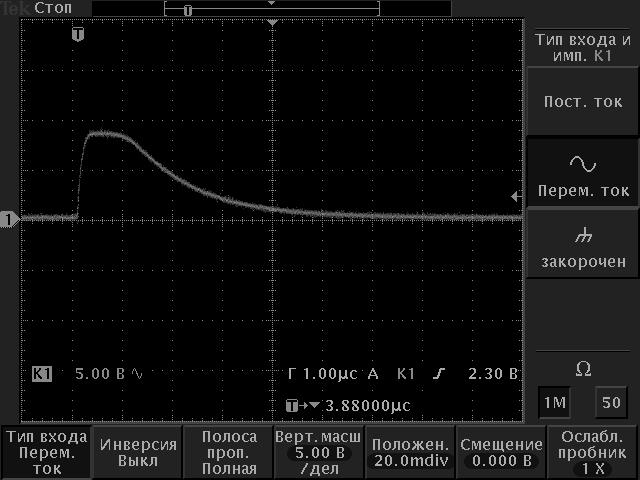
\includegraphics[width=0.5\textwidth]{LEMPH Report_files/LEMPH Report_66_0.jpeg}
    \par
    \end{center}
    

            
        
    
\subsection{Спектры различных источников}
        

        \renewcommand{\indexname}{Index}
  

    % End of document
    \end{document}


